\documentclass[hyphens,aspectratio=169,dvipsnames]{beamer}
\usepackage{graphicx}
\usepackage{xcolor}
\usepackage{amssymb}
\usepackage{amsmath}
\usepackage{mathtools}
\usepackage{textcomp}
\usepackage{moresize}
\usepackage{framed}
\usepackage{minted}
\usepackage{relsize}
\usepackage{tikz}
\usepackage{comment}
\usetikzlibrary{shapes.geometric, arrows, positioning}
\usetheme{Berlin}
\usecolortheme[RGB={0,95,47}]{structure}
\beamertemplatenavigationsymbolsempty

\makeatletter
\AtBeginEnvironment{minted}{\dontdofcolorbox}
\def\dontdofcolorbox{\renewcommand\fcolorbox[4][]{##4}}
\makeatother

\newcommand{\textpf}[1]{\texttt{\color{black}\fcolorbox{lightgray}{lightgray}{#1}}}

\begin{document}

\begin{frame}{Questions}
    \begin{itemize}
        \pause \item I've attempted to make today's lecture a little lighter so that I can better address some things covered in the last class.
        \pause \item As always, feel free to interrupt with questions, even if they're about past classes' material.
    \end{itemize}
\end{frame}

\begin{frame}{CPU Privelege Levels}
    \begin{itemize}
        \pause \item x86\_64 CPUs have two primary privilege levels: ring 0 (kernel) and ring 3 (user).
        \pause \item When a CPU is executing in ring 3, it is in its least priveleged state.
        \pause \item When a CPU is executing in ring 0, it is in its most priveleged state.
    \end{itemize}
\end{frame}

\begin{frame}{}
    \begin{center}
        \begin{tabular}{c c}
            Ring 3 & Ring 0 \\
            
\includegraphics[height=0.3\textwidth]{davey.jpeg} & 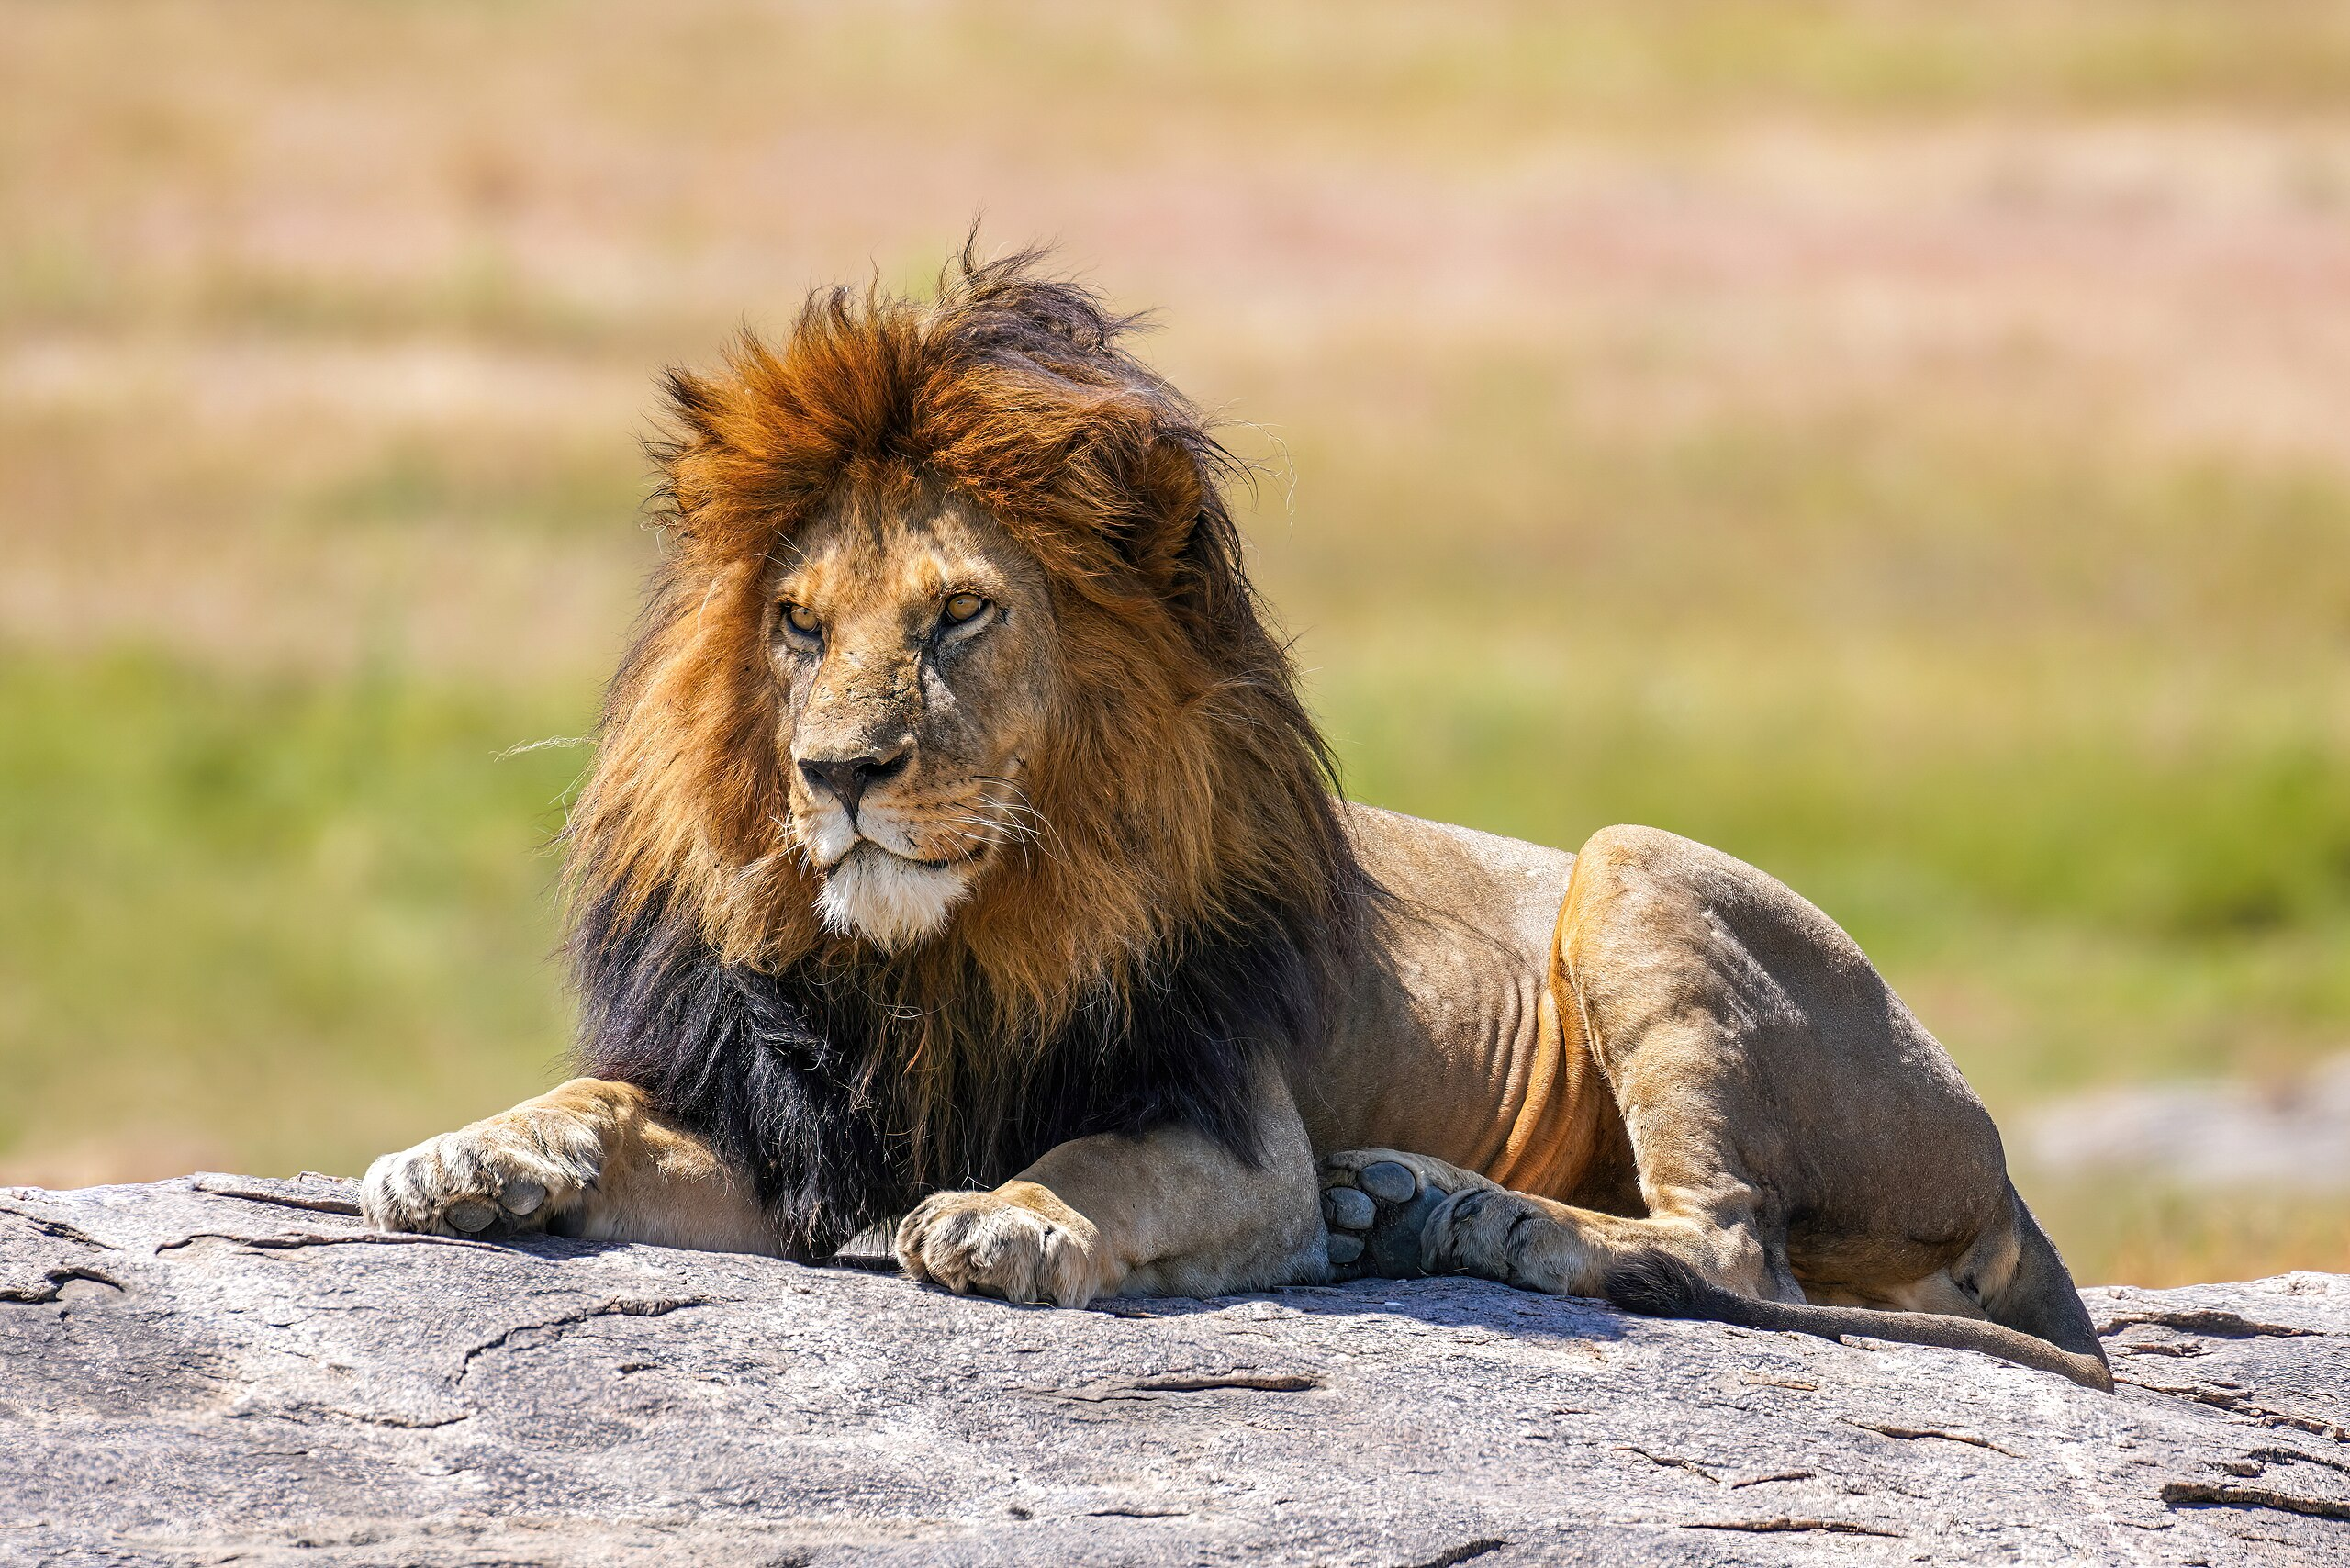
\includegraphics[height=0.3\textwidth]{lion.jpg}
        \end{tabular}
    \end{center}
\end{frame}

\begin{frame}{Ring 3}
    \begin{itemize}
        \pause \item All the code you have ever run on an x86\_64 CPU has been in ring 3.
        \pause \item Even when you're \texttt{root}, you're still in ring 3.
    \end{itemize}
\end{frame}

\begin{frame}{Ring 0}
    Much of the interesting stuff that computers do can only be done from ring 0.
    This includes
    \begin{itemize}
        \pause \item Sending/receiving data over the network
        \pause \item Reading/writing to/from files
        \pause \item Printing stuff to \textpf{stdout}
        \pause \item Interacting with peripherals
    \end{itemize}
\end{frame}

\begin{frame}{Accessing Ring 0 from Ring 3}
    \begin{itemize}
        \pause \item If all those things require ring 0 privileges, and your code runs in ring 3, how is your code able to do those things?
        \pause \item System calls!
    \end{itemize}
\end{frame}

\begin{frame}{System Calls}
    \begin{itemize}
        \pause \item System calls (a.k.a. syscalls) are how user programs ask the kernel to do privileged operations.
        \pause \item Each syscall has a unique \textit{syscall number}.
    \end{itemize}

    For example,
    \begin{itemize}
        \pause \item The \texttt{read} syscall (x86\_64 syscall number 0) reads from a file descriptor.
        \pause \item The \texttt{write} syscall (x86\_64 syscall number 1) writes to a file descriptor.
        \pause \item The \texttt{open} syscall (x86\_64 syscall number 2) acquires a file descriptor for a provided file path.
        \pause \item The \texttt{close} syscall (x86\_64 syscall number 3) closes an existing file descriptor.
        \pause \item The \texttt{exit} syscall (x86\_64 syscall number 60) exits the process.
    \end{itemize}
\end{frame}

\begin{frame}{Making a System Call}
    \begin{itemize}
        \pause \item To make a system call, use the \textpf{syscall} libc function, provided by \textpf{<unistd.h>}.
        \pause \item The first argument to this function is the syscall number of the system call you'd like to invoke.
        \pause \item The rest of the arguments depend on which system call you're invoking.
        \pause \item Consult this giant table for more details:
        \pause \item \url{https://www.chromium.org/chromium-os/developer-library/reference/linux-constants/syscalls/}
    \end{itemize}
\end{frame}

\begin{frame}{Example: Nonportable \textpf{exit}}
    \inputminted{c}{./exit_55.c}
\end{frame}

\begin{frame}{Portability}
    \begin{itemize}
        \pause \item On other OSes, and even on some other Linux machines, the \textpf{exit} syscall will have a different syscall number.
        \pause \item For this reason, it's best to use the \textpf{SYS\_*} constants defined in \textpf{<sys/syscall.h>} when possible.
    \end{itemize}
\end{frame}

\begin{frame}{Example: Portable \textpf{exit}}
    \inputminted{c}{./exit_55_portable.c}
\end{frame}

\begin{frame}{File Descriptors}
    \begin{itemize}
        \pause \item On Unix, there are 3 file descriptors that are open when a process starts:
            \begin{itemize}
                \pause \item \textpf{stdin}, file descriptor 0
                \pause \item \textpf{stdout}, file descriptor 1
                \pause \item \textpf{stderr} file descriptor 2
            \end{itemize}
        \pause \item In order to perform operations on a file, you first need to acquire a file descriptor using the \textpf{open} system call.
    \end{itemize}
\end{frame}

\begin{frame}{Activity: DIY \textpf{cat}}
    \begin{itemize}
        \pause \item Write a C program that makes a \textpf{write} system call to write something cool to \textpf{stdout}.
        \pause \item Modify your program to read $\leq 100$ bytes from \textpf{stdin}, and \textpf{write} the received data to \textpf{stdout}.
        \pause \item Modify your program to repeatedly \textpf{read} and \textpf{write} in a loop until either system call fails.
        \pause \item Make a new file called \textpf{prog\_input}. Modify your program to read from that file instead of \textpf{stdin}.
    \end{itemize}
\end{frame}

\begin{frame}{Strings}
    \begin{itemize}
        \pause \item Strings are just \textpf{char *}s.
        \pause \item Because \textpf{sizeof} doesn't work on pointers, you need some other way of knowing when a string ends.
        \pause \item One way to do this is to store strings along with their lengths.
        \pause \item Another way to do this is to designate some byte (or byte sequence) as meaning ``end of string."
        \pause \item In C, it's traditional to use the 0 byte for this purpose.
    \end{itemize}
\end{frame}

\begin{frame}{Activity: Character Count}
    \begin{itemize}
        \pause \item Write a function \textpf{unsigned long char\_count(char *s, char c)} that counts the number of occurrences of the \textpf{char} \textpf{c} in the string \textpf{s}.
        \pause \item Verify that your function works on reasonable arguments, then try passing weird arguments to your function. What does it do?
    \end{itemize}
\end{frame}

\end{document}
